\documentclass[a4paper, ngerman]{scrartcl}

%\usepackage[T1]{fontenc}
%\usepackage[utf8]{inputenc}
\usepackage[ngerman]{babel}
\usepackage{lmodern}
\usepackage{hyperref}
\usepackage{graphicx}
\usepackage{paralist}
\usepackage{wrapfig}
\usepackage{float} % enables usage of H parameter in figures which means "really here"
\usepackage[font=small,skip=8pt]{caption} % reduce space between caption and figure

% for the copyright notice
\newcommand\blfootnote[1]{%
  \begingroup
  \renewcommand\thefootnote{}\footnote{#1}%
  \addtocounter{footnote}{-1}%
  \endgroup
}

\hypersetup{
  pdfborder = {0 0 0},
  urlbordercolor = {0 0 0},
  colorlinks = true,
  linkcolor = black,
  citecolor = black,
  filecolor = black,
  urlcolor  = black
}

\usepackage{fontspec}
%\setromanfont{Merriweather}
%\setsansfont{Lato}


\titlehead{\centering
\includegraphics[width=3.5cm]{bilder/logo.png}}
\subject{Software-Challenge 2016}
\title{Spielregeln}
\subtitle{Twixt}
\date{Stand: \today}

\begin{document}


\maketitle

\begin{figure}[!htbp]
  \centering
  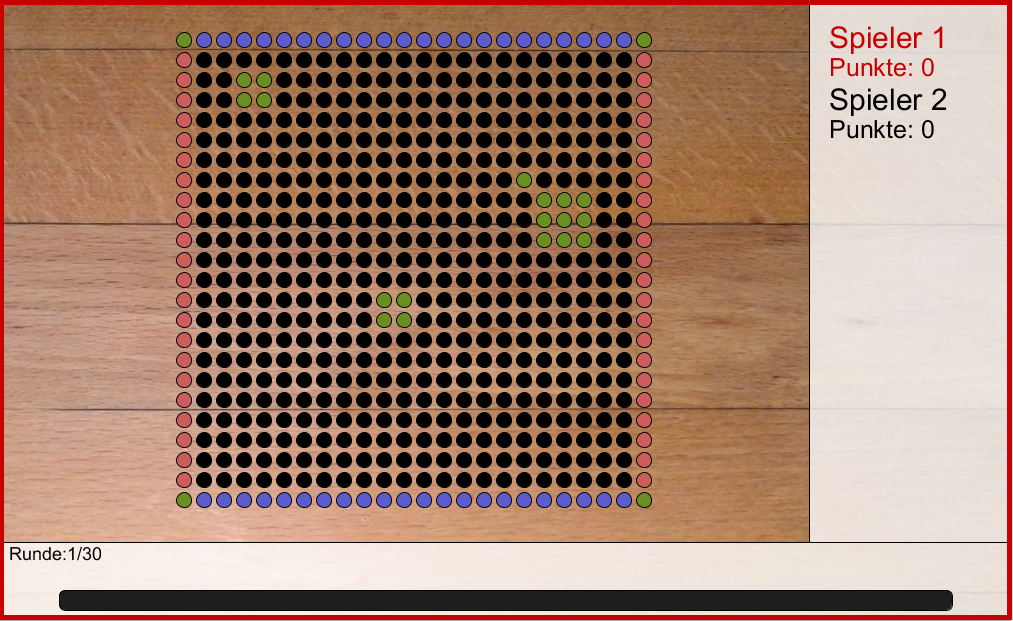
\includegraphics[width=\linewidth]{bilder/gui.png}
\end{figure}
\vspace*{\fill}

\blfootnote{Die Nutzung des Spielkonzeptes "`Twixt"' (Name, Spielregeln und Grafik)
  erfolgt mit freundlicher Genehmigung des Kosmos Verlags.}

\newpage

\section{Einführung}

In dieser Anleitung werden die Elemente und Regeln des Spiels \emph{Twixt} der
Software-Challenge 2016 erläutert.

Bei Twixt versuchen zwei Spieler, durch abwechselndes setzen von Strommasten
eine durchgehende Verbindung zwischen den beiden gegenüberliegenden Spielfeldrändern
herzustellen, und gleichzeitig den Gegenspieler daran zu hindern, das Gleiche zu
tun.

\section{Das Spielbrett}
Das Spielbrett ist im Titelbild zu sehen und besteht aus 576 Feldern.
Mit Ausnahme der Sumpffelder (grün) kann auf jedes dieser Felder genau 
ein Strommast gestellt werden. Allerdings kann Blau keine Strommasten auf 
die oberen und unteren Randfelder (rot) stellen und Rot nicht auf die linken 
und rechten Randfelder (blau). In den 4 Ecken befindet sich jeweils ein
Sumpffeld.
Zusätzlich werden vor Spielbeginn 4 Sümpfe zufällig generiert. Dabei handelt sich um 
ein einzelnes Sumpffeld, zwei mittelgroße Sümpfe mit jeweils 2x2 Sumpffeldern 
sowie einen großen Sumpf mit 3x3 Sumpffeldern. Keines der zufällig generierten Sumpffelder 
befindet sich auf einem Rand- oder Eckfeld. Die zufällig generierten Sümpfe dürfen 
sich jedoch überschneiden.

\begin{wrapfigure}{r}{0.5\textwidth}
  \centering
  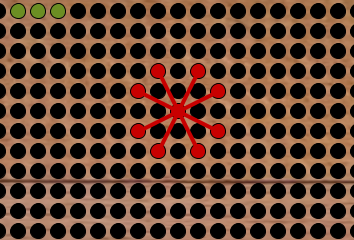
\includegraphics[width=0.48\textwidth]{bilder/setzzug.png}
  \caption{Alle möglichen Leitungen}\label{fig:Leitungen}
\end{wrapfigure}

\section{Der Spielablauf}
Zu Beginn des Spiels setzt zunächst Rot einen neuen Strommast auf ein
freies Feld, also ein Feld, das weder ein Sumpffeld noch ein Feld der
gegnerischen Farbe ist und auf dem sich noch kein Strommast befindet.
Danach tut Blau dasselbe, während beide versuchen,
ihre beiden Farbzonen (farbig markierte Felder; für Rot sind diese oben und
unten, für Blau  links und rechts) mit einer zusammenhängenden Leitung zu
verbinden.

Bei einem Zug ist es möglich, dass sich dadurch eine oder mehrere
neue Leitungen bilden. Eine neue Leitung bildet sich, wenn sich ein eigener
Strommast in folgendem Abstand zu dem gesetztem Strommast befindet: Zwei
waagerecht und ein Feld senkrecht oder eins waagerecht und zwei Felder
senkrecht. Dies geschieht aber nur, wenn bisher keine Leitung existiert, die
die entstehende Leitung kreuzen würde.
Ein Beispiel, welche Leitungen von einem Strommast aus möglich sind, ist
in Abbildung 1 zu sehen.


\section{Ende des Spiels}
Das Spiel endet, sobald es einer der Spieler geschafft hat, seine beiden
Farbzonen mit einer zusammenhängenden Leitung zu verbinden, spätestens jedoch
nach 30 Runden.

Für die Berechnung der Punkte von Rot ist allein diejenige zusammenhängende
Leitung von Rot entscheidend, welche in vertikaler Richtung die längste
Ausdehnung hat. Die Ausdehnung dieser Leitung in vertikaler Richtung ergibt
die Punktezahl für Rot. Entsprechend zählt für Blau die horizontale Ausdehnung.
In dem in Abbildung 2 gezeigten Beispiel erhält Rot deshalb 8 Punkte (es zählt ausschließlich
die vertikale Richtung)
und Blau 4 (die kürzere Leitung zählt nicht). Das Spiel gewinnt derjenige Spieler, der am Spielende
die meisten Punkte hat.
Ist die so ermittelte Punktzahl gleich, ist das Ergebnis unentschieden.

\section{Die graphische Benutzeroberfläche}

Beim Start des graphischen Servers wird das Hauptfenster angezeigt,
welches bis zum Start eines Spiels aber leer bleibt. Die folgenden
Beschreibungen gehen davon aus, dass ein Twixt-Spiel gestartet wurde.

\subsection{Das Hauptfenster}

\begin{figure}[H]
  \centering
  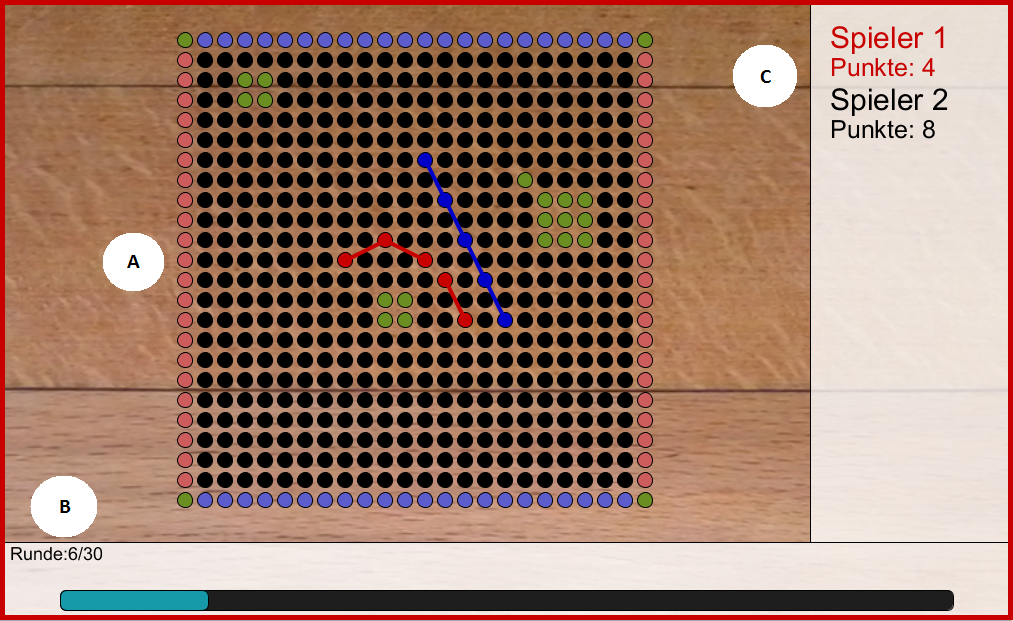
\includegraphics[width=0.8\textwidth]{bilder/uebersicht.png}
  \caption{Überblick der GUI}\label{fig:GUI}
\end{figure}

\begin{minipage}{\linewidth} % using minipage to prevent pagebreak in list
In Abbildung~\ref{fig:GUI} ist ein Überblick der graphischen Benutzeroberfläche
zu sehen. Die markanten Spielelemente sind mit \emph{A-C} gekennzeichnet.

\begin{compactenum}[A)]
\item Das Spielbrett
\item Die Spielfortschrittsanzeige 
\item Der Punktestand der Spieler
\end{compactenum}
\end{minipage}

\subsection{Das Einstellungsmenü}

\begin{wrapfigure}{l}{0.5\textwidth}
  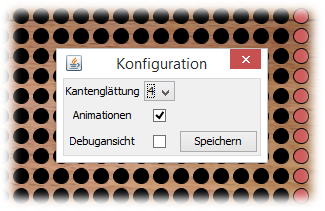
\includegraphics[width=0.48\textwidth]{bilder/konfiguration.png}
  \centering
  \caption{Das Einstellungsmenü}\label{fig:Configuration}
\end{wrapfigure}

Ein Einstellungsmenü mit Darstellungsoptionen wird in Abbildung 3
dargestellt und lässt sich über die Taste 'C' anzeigen. Dazu muss das
Spielfeld den Tastaturfokus haben (erforderlichenfalls vorher
Mausklick auf das Spielfeld). Es stehen dort folgende Einstellungen
zur Verfügung:

\textbf{Kantenglättung} verbessert die Optik des
Spiels, ist aber rechenintensiv, diese hat Einstellungen von 0 bis 8 und ist
standardmäßig auf 4 gestellt.
Auf sehr langsamen Rechnern sollte sie daher auf 0 gestellt werden. Die Option
Die \textbf{Debugansicht} zeigt Debug-Hilfestellungen zu einzelnen Zügen und
die Framerate an.
Diese Hilfestellungen sind Texte, die ein Spielclient einem Zug beifügen kann, den er
an den Spielserver sendet.

\end{document}
